% The package inside an ordinary article: loaded after xcolor with options and
% alongside hyperref (no option clash), a diagram inline in an equation -- the
% same expansion twice, once drawn downward and once along the line.
%
% The horizontal one is the one to copy for running text: it is one stack, so
% it is centered on y = 0, and `baseline=-0.5ex' puts that line on the math
% axis, where the = and the \psi beside it sit. Nothing else in it is placed.
\documentclass{article}
\usepackage[dvipsnames]{xcolor}
\usepackage{amsmath}
\usepackage{tikz-tensors}
\input{notation}
\usepackage{hyperref}
\pagestyle{empty}
\begin{document}
\[
  \psi(\mathbf r_1, \mathbf r_2) \;=\;
  \begin{tikzpicture}[baseline=-1.2cm]
    \node[coefwide] (C) at (0,0) {$C$};
    \node[fn] (a) at (-0.45,-1.3) {$\varphi$};
    \node[fn] (b) at ( 0.45,-1.3) {$\varphi$};
    \draw[disc] (C.south -| a) -- (a);
    \draw[disc] (C.south -| b) -- (b);
    \draw[cont] (a.south) -- ++(0,-0.8) node[leg, below] {$\mathbf r_1$};
    \draw[cont] (b.south) -- ++(0,-0.8) node[leg, below] {$\mathbf r_2$};
  \end{tikzpicture}
  \quad\text{in {\color{ForestGreen}text} and {\color{ele}ele}.}
\]
\[
  \psi(\mathbf r_1, \mathbf r_2) \;=\;
  \begin{tikzpicture}[baseline=-0.5ex]
    \tnstack{X}{3}{ket}
    \tnlayer{X}{ket}{fn/$\varphi$, coef/$C$, fn/$\varphi$}
    \tnconnect{X}
    \tnopen[edge=cont, label=$\mathbf r_1$]{left}{X-ket-1}
    \tnopen[edge=cont, label=$\mathbf r_2$]{right}{X-ket-3}
  \end{tikzpicture}
  \quad\text{along the line.}
\]
\end{document}
